\documentclass{standalone}
\usepackage{tikz}
\usetikzlibrary{patterns, positioning}

\begin{document}
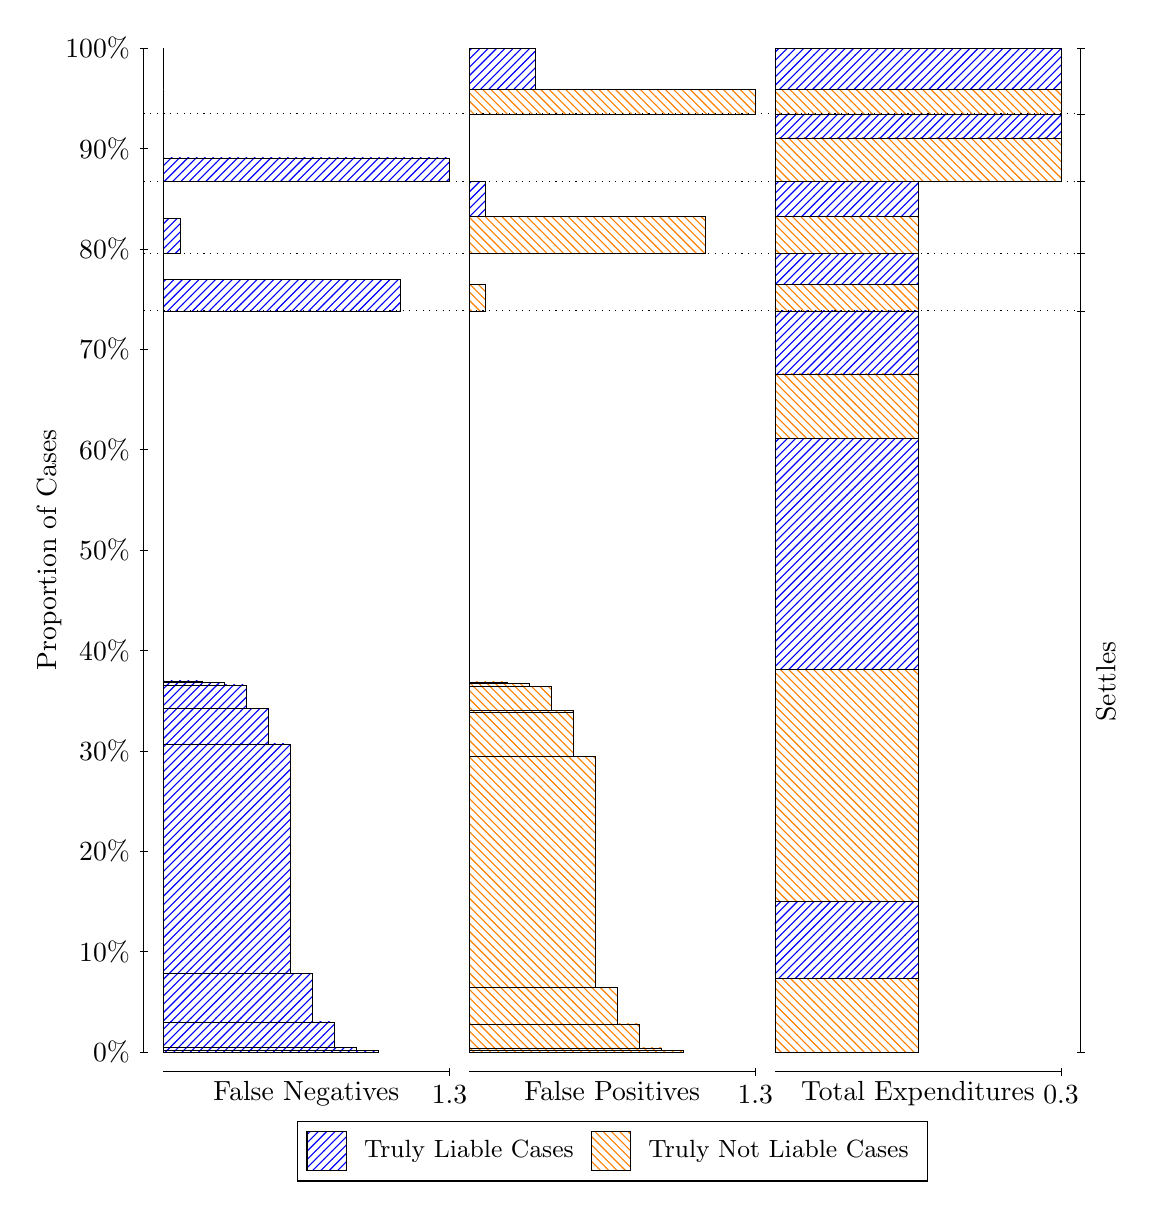
\begin{tikzpicture}
\draw[black, very thin] (1.5,1.75) -- (1.5,14.5);
\node[rotate=90, anchor=center] at (0.3, 8.125) {Proportion of Cases};
\draw[black, very thin] (1.45,1.75) -- (1.55,1.75);
\node[anchor=east] at (1.45, 1.75) {0\%};
\draw[black, very thin] (1.45,3.025) -- (1.55,3.025);
\node[anchor=east] at (1.45, 3.025) {10\%};
\draw[black, very thin] (1.45,4.3) -- (1.55,4.3);
\node[anchor=east] at (1.45, 4.3) {20\%};
\draw[black, very thin] (1.45,5.575) -- (1.55,5.575);
\node[anchor=east] at (1.45, 5.575) {30\%};
\draw[black, very thin] (1.45,6.85) -- (1.55,6.85);
\node[anchor=east] at (1.45, 6.85) {40\%};
\draw[black, very thin] (1.45,8.125) -- (1.55,8.125);
\node[anchor=east] at (1.45, 8.125) {50\%};
\draw[black, very thin] (1.45,9.4) -- (1.55,9.4);
\node[anchor=east] at (1.45, 9.4) {60\%};
\draw[black, very thin] (1.45,10.675) -- (1.55,10.675);
\node[anchor=east] at (1.45, 10.675) {70\%};
\draw[black, very thin] (1.45,11.95) -- (1.55,11.95);
\node[anchor=east] at (1.45, 11.95) {80\%};
\draw[black, very thin] (1.45,13.225) -- (1.55,13.225);
\node[anchor=east] at (1.45, 13.225) {90\%};
\draw[black, very thin] (1.45,14.5) -- (1.55,14.5);
\node[anchor=east] at (1.45, 14.5) {100\%};

\draw[black, very thin] (13.4,1.75) -- (13.4,14.5);
\draw[black, very thin] (13.35,1.75) -- (13.45,1.75);
\node[anchor=west] at (13.35, 1.75) {};
\draw[black, very thin] (13.35,11.162) -- (13.45,11.162);
\node[anchor=west] at (13.35, 11.162) {};
\draw[black, very thin] (13.35,11.896) -- (13.45,11.896);
\node[anchor=west] at (13.35, 11.896) {};
\draw[black, very thin] (13.35,12.803) -- (13.45,12.803);
\node[anchor=west] at (13.35, 12.803) {};
\draw[black, very thin] (13.35,13.663) -- (13.45,13.663);
\node[anchor=west] at (13.35, 13.663) {};
\draw[black, very thin] (13.35,14.5) -- (13.45,14.5);
\node[anchor=west] at (13.35, 14.5) {};

\draw[black, very thin, pattern color=blue, pattern=north east lines] (1.75,1.75) rectangle (4.475,1.7674);
\draw[black, very thin, pattern color=blue, pattern=north east lines] (1.75,1.7674) rectangle (4.1955,1.8092);
\draw[black, very thin, pattern color=blue, pattern=north east lines] (1.75,1.8092) rectangle (3.916,2.1325);
\draw[black, very thin, pattern color=blue, pattern=north east lines] (1.75,2.1325) rectangle (3.6365,2.7457);
\draw[black, very thin, pattern color=blue, pattern=north east lines] (1.75,2.7457) rectangle (3.3571,5.6618);
\draw[black, very thin, pattern color=blue, pattern=north east lines] (1.75,5.6618) rectangle (3.0776,6.1183);
\draw[black, very thin, pattern color=blue, pattern=north east lines] (1.75,6.1183) rectangle (2.7981,6.4127);
\draw[black, very thin, pattern color=blue, pattern=north east lines] (1.75,6.4127) rectangle (2.5186,6.4459);
\draw[black, very thin, pattern color=blue, pattern=north east lines] (1.75,6.4459) rectangle (2.2391,6.4628);
\draw[black, very thin, pattern color=orange, pattern=north west lines] (1.75,6.4628) rectangle (1.75,11.162);
\draw[black, very thin, pattern color=blue, pattern=north east lines] (1.75,11.162) rectangle (4.7545,11.558);
\draw[black, very thin, pattern color=orange, pattern=north west lines] (1.75,11.558) rectangle (1.75,11.896);
\draw[black, very thin, pattern color=blue, pattern=north east lines] (1.75,11.896) rectangle (1.9596,12.336);
\draw[black, very thin, pattern color=orange, pattern=north west lines] (1.75,12.336) rectangle (1.75,12.803);
\draw[black, very thin, pattern color=blue, pattern=north east lines] (1.75,12.803) rectangle (5.3833,13.105);
\draw[black, very thin, pattern color=orange, pattern=north west lines] (1.75,13.105) rectangle (1.75,13.663);
\draw[black, very thin, pattern color=orange, pattern=north west lines] (1.75,13.663) rectangle (1.75,13.975);
\draw[black, very thin, pattern color=blue, pattern=north east lines] (1.75,13.975) rectangle (1.75,14.5);
\draw[black, very thin, pattern color=orange, pattern=north west lines] (5.6333,1.75) rectangle (8.3583,1.7658);
\draw[black, very thin, pattern color=orange, pattern=north west lines] (5.6333,1.7658) rectangle (8.0788,1.8015);
\draw[black, very thin, pattern color=orange, pattern=north west lines] (5.6333,1.8015) rectangle (7.7994,2.1056);
\draw[black, very thin, pattern color=orange, pattern=north west lines] (5.6333,2.1056) rectangle (7.5199,2.568);
\draw[black, very thin, pattern color=orange, pattern=north west lines] (5.6333,2.568) rectangle (7.2404,5.4997);
\draw[black, very thin, pattern color=orange, pattern=north west lines] (5.6333,5.4997) rectangle (6.9609,6.0653);
\draw[black, very thin, pattern color=orange, pattern=north west lines] (5.6333,6.0653) rectangle (6.9609,6.0926);
\draw[black, very thin, pattern color=orange, pattern=north west lines] (5.6333,6.0926) rectangle (6.6814,6.3951);
\draw[black, very thin, pattern color=orange, pattern=north west lines] (5.6333,6.3951) rectangle (6.4019,6.4334);
\draw[black, very thin, pattern color=orange, pattern=north west lines] (5.6333,6.4334) rectangle (6.1224,6.4495);
\draw[black, very thin, pattern color=blue, pattern=north east lines] (5.6333,6.4495) rectangle (5.6333,11.162);
\draw[black, very thin, pattern color=orange, pattern=north west lines] (5.6333,11.162) rectangle (5.8429,11.5);
\draw[black, very thin, pattern color=blue, pattern=north east lines] (5.6333,11.5) rectangle (5.6333,11.896);
\draw[black, very thin, pattern color=orange, pattern=north west lines] (5.6333,11.896) rectangle (8.6378,12.364);
\draw[black, very thin, pattern color=blue, pattern=north east lines] (5.6333,12.364) rectangle (5.8429,12.803);
\draw[black, very thin, pattern color=orange, pattern=north west lines] (5.6333,12.803) rectangle (5.6333,13.36);
\draw[black, very thin, pattern color=blue, pattern=north east lines] (5.6333,13.36) rectangle (5.6333,13.663);
\draw[black, very thin, pattern color=orange, pattern=north west lines] (5.6333,13.663) rectangle (9.2667,13.975);
\draw[black, very thin, pattern color=blue, pattern=north east lines] (5.6333,13.975) rectangle (6.4718,14.5);
\draw[black, very thin, pattern color=orange, pattern=north west lines] (9.5167,1.75) rectangle (11.333,2.6837);
\draw[black, very thin, pattern color=blue, pattern=north east lines] (9.5167,2.6837) rectangle (11.333,3.662);
\draw[black, very thin, pattern color=orange, pattern=north west lines] (9.5167,3.662) rectangle (11.333,6.6099);
\draw[black, very thin, pattern color=blue, pattern=north east lines] (9.5167,6.6099) rectangle (11.333,9.5433);
\draw[black, very thin, pattern color=orange, pattern=north west lines] (9.5167,9.5433) rectangle (11.333,10.361);
\draw[black, very thin, pattern color=blue, pattern=north east lines] (9.5167,10.361) rectangle (11.333,11.162);
\draw[black, very thin, pattern color=orange, pattern=north west lines] (9.5167,11.162) rectangle (11.333,11.5);
\draw[black, very thin, pattern color=blue, pattern=north east lines] (9.5167,11.5) rectangle (11.333,11.896);
\draw[black, very thin, pattern color=orange, pattern=north west lines] (9.5167,11.896) rectangle (11.333,12.364);
\draw[black, very thin, pattern color=blue, pattern=north east lines] (9.5167,12.364) rectangle (11.333,12.803);
\draw[black, very thin, pattern color=orange, pattern=north west lines] (9.5167,12.803) rectangle (13.15,13.36);
\draw[black, very thin, pattern color=blue, pattern=north east lines] (9.5167,13.36) rectangle (13.15,13.663);
\draw[black, very thin, pattern color=orange, pattern=north west lines] (9.5167,13.663) rectangle (13.15,13.975);
\draw[black, very thin, pattern color=blue, pattern=north east lines] (9.5167,13.975) rectangle (13.15,14.5);
\draw[black, dotted] (1.5,11.162) -- (13.4,11.162);
\draw[black, dotted] (1.5,11.896) -- (13.4,11.896);
\draw[black, dotted] (1.5,12.803) -- (13.4,12.803);
\draw[black, dotted] (1.5,13.663) -- (13.4,13.663);
\draw[black, very thin] (1.75,1.5) -- (5.3833,1.5);
\node[anchor=north] at (3.5667, 1.5) {False Negatives};
\draw[black, very thin] (5.3833,1.45) -- (5.3833,1.55);
\node[anchor=north] at (5.3833, 1.45) {1.3};

\draw[black, very thin] (5.6333,1.5) -- (9.2667,1.5);
\node[anchor=north] at (7.45, 1.5) {False Positives};
\draw[black, very thin] (9.2667,1.45) -- (9.2667,1.55);
\node[anchor=north] at (9.2667, 1.45) {1.3};

\draw[black, very thin] (9.5167,1.5) -- (13.15,1.5);
\node[anchor=north] at (11.333, 1.5) {Total Expenditures};
\draw[black, very thin] (13.15,1.45) -- (13.15,1.55);
\node[anchor=north] at (13.15, 1.45) {0.3};

\node[black, centered, rotate=90] at (13.72, 6.4562) {Settles};





\draw (7.449999999999999,1.5) node[draw=none] (baseCoordinate) {};
\begin{scope}[align=center]
        \matrix[scale=0.5, draw=black, below=0.5cm of baseCoordinate, nodes={draw}, column sep=0.1cm]{
            \node[rectangle, draw, minimum width=0.5cm, minimum height=0.5cm, pattern=north east lines, pattern color=blue] {}; &
            \node[draw=none, font=\small] (B) {Truly Liable Cases}; &
            \node[rectangle, draw, minimum width=0.5cm, minimum height=0.5cm, pattern=north west lines, pattern color=orange] {}; &
            \node[draw=none, font=\small] (B) {Truly Not Liable Cases}; \\
            };
\end{scope}

\end{tikzpicture}
\end{document}